\documentclass[aps,prl,preprint,groupedaddress]{revtex4}
%\documentclass[aps,prl,twocolumn,groupedaddress]{revtex4}

\usepackage[dvips]{graphicx,color} % Graphics and color
\usepackage{array,hhline,dcolumn} % Better table handling
\usepackage{rotating} % Rotate and sideways environments
%\usepackage(lineno)
\usepackage{amssymb,amsmath}


\bibliographystyle{unsrt} % For BibTeX - sorted numerical labels by
                                % order of first citation.


% Useful commands.
%\input{commands}
\newcommand{\ie}{\sl i.e.}
\newcommand{\kov}{$\check\mathrm{C}$erenkov }
\newcommand{\hz}{\,\mathrm{Hz}}
\newcommand{\khz}{\,\mathrm{kHz}}
\newcommand{\mhz}{\,\mathrm{MHz}}
\newcommand{\kev}{\,\mathrm{keV}}
\newcommand{\mev}{\,\mathrm{MeV}}
\newcommand{\mevc}{\,\mathrm{MeV}/c}
\newcommand{\mevcc}{\,\mathrm{MeV}/c^2}
\newcommand{\gev}{\,\mathrm{GeV}}
\newcommand{\cmsq}{\,\mathrm{cm}^2}
\newcommand{\nm}{\,\mathrm{nm}}
\newcommand{\ms}{\,\mathrm{m}}
\newcommand{\msec}{\,\mathrm{ms}}
\newcommand{\nsec}{\,\mathrm{ns}}
\newcommand{\dmsq}{\Delta m^{2}~}
\newcommand{\musec}{\mu s}
\newcommand{\nubar}{\bar{\nu}}
\newcommand{\numu}{\nu_{\mu}}
\newcommand{\numubar}{\bar{\nu}_{\mu}}
\newcommand{\nue}{\nu_e}
\newcommand{\nuebar}{\bar{\nu}_e}
\newcommand{\nutau}{\nu_{\tau}}
\newcommand{\nux}{\nu_x}
\newcommand{\nuxbar}{\bar{\nu}_x}
\newcommand{\mutoe}{\numu\rightarrow\nue}
\newcommand{\mubartoebar}{\numubar\rightarrow\nuebar}
\newcommand{\mutotau}{\numu\rightarrow\nutau}
\newcommand{\mutox}{\numu\rightarrow\nux}
\newcommand{\mubartoxbar}{\numubar\rightarrow\nuxbar}
\newcommand{\piplusdecay}{\pi^+ \rightarrow \mu^+ \numu}
\newcommand{\piminusdecay}{\pi^- \rightarrow \mu^- \numubar}
\newcommand{\pimue}{\pi \rightarrow \mu \rightarrow e}
\newcommand{\muplusdecay}{\mu^+ \rightarrow e^+ \nue \numubar}
\newcommand{\muminusdecay}{\mu^- \rightarrow e^- \nuebar \numu}
\newcommand{\sinsqtheta}{\sin^2 2 \theta~}
\newcommand{\pizero}{\pi^{0}}
\newcommand{\pip}{\pi^{+}}
\newcommand{\pim}{\pi^{-}}
\newcommand{\pipm}{\pi^{\pm}}
\newcommand{\Kp}{K^{+}}
\newcommand{\Km}{K^{-}}
\newcommand{\KL}{K^{0}_{L}}
\newcommand{\KS}{K^{0}_{S}}
\newcommand{\reaction}{\nuebar + p \to e^{+} + n\ \ \ ,}
\newcommand{\evsq}{{eV}^{2}}
\newcommand{\flux}{\,\nu/\mathrm{cm}^{2}/p}
\newcommand{\barflux}{\,\bar \nu/\mathrm{cm}^{2}/p}
\newcommand{\ga}{\gamma}
\newcommand{\gtwid}{\mathrel{\raise.3ex\hbox{$>$\kern-.75em\lower1ex\hbox{$\sim$}}}}
\newcommand{\ltwid}{\mathrel{\raise.3ex\hbox{$<$\kern-.75em\lower1ex\hbox{$\sim$}}}}

\newcommand{\datapot}{6.023\times10^{20}}
\newcommand{\nveto}{N_{VETO}}
\newcommand{\ntank}{N_{TANK}}
\newcommand{\demu}{-\log(L_e/L_\mu)}
\newcommand{\depifr}{-\log(L_e/L_\pi(fr))}
\newcommand{\depifx}{-\log(L_e/L_\pi(fx))}

%%%%%%%%%%%%%%%%%%%%%%%%%%%%%%%%%%%%%%%%%%%%%%%%%%%%%%%%%%%%%%%%%%%%%%%%%%
%   To make a draft of only one or several sections, uncomment the line  %
%   below and put in the desired section(s).  Note: if you LaTex the     %
%   whole document once first, LaTex remembers the right page numbers,   %
%   etc!
%%%%%%%%%%%%%%%%%%%%%%%%%%%%%%%%%%%%%%%%%%%%%%%%%%%%%%%%%%%%%%%%%%%%%%%%%%
%\includeonly{onesection,anothersection}
%\includeonly{oscillation_search}
% Main document
\begin{document}
%\countdef\pageno=0 \pageno=105
%\voffset=0.75in
%
%Below writes "DRAFT"
%\special{!userdict begin /bop-hook{gsave 200 30 translate
%65 rotate /Times-Roman findfont 216 scalefont setfont
%0 0 moveto 0.7 setgray (DRAFT) show grestore} def end}
% APS preprint designation
% \preprint{MiniBooNE-OSC}

\centerline{\bf LBNE Fine-Grained-Tracker Near Detector}
\smallskip
\centerline{December 18, 2013}

\bigskip

\section{Abstract}

The LBNE Fine-Grained-Tracker (FGT) near detector design has been jointly
developed with US and Indian institutions. The FGT consists of a straw-tube
tracking detector (STT) and electromagnetic calorimeter (ECAL) inside of a 0.4 T
dipole magnet. In addition, Muon Identifiers (MuIDs) are located in the
steel of the magnet, as well as upstream and downstream of the STT. The FGT
is designed to make precision measurements of the neutrino fluxes and 
cross sections. 
In the Proposal of Indian Institutions and Fermilab Collaboration (IIFC) for Participation in 
the Long-Baseline Neutrino Experiment at Fermilab 
(12 December 2012), it is proposed that India build the FGT to enhance the capabilities of the 
overall LBNE scientific program. 
This document presents an overview of the FGT design, which 
will meet the physics goals and sensitivities presented in the IIFC proposal. The document 
summarizes the deliverables from the Indian institutions. More details can be found in the full Proposal above.

\section{Motivation}

In order for LBNE to achieve the desired neutrino-oscillation sensitivity, the 
charged-current signal events
and neutral-current
background events in the LBNE far detector (FD) must be precisely 
predicted as a function of the parameters and variables that affect 
oscillations. These include energy, leading lepton (which tags the neutrino flavor) and the 
momentum and identification of particles generated by neutrino interactions. 
It is, therefore, crucial to measure the un-oscillated neutrino fluxes and 
their interactions at the near site. At the FD, the first and the second 
oscillation maxima signals occur at about 2.4 GeV and 0.8 GeV, respectively 
-- an energy regime where neutrino cross sections and fluxes have large 
uncertainties. 

In addition to the oscillation signal, it is 
critical to identify and measure processes such as neutral current $\pi^0$ production,
that can mimic oscillation signals 
at the FD. Thus, the principal focus of the neutrino detector will be 
on the neutrino-oscillation energy range of $E_\nu < 8$ GeV, as well as higher 
neutrino energies that produce background to the oscillation signal. Furthermore, the
$8<E_\nu < 20$ GeV energy range can be used as a ``control region'' or
as a region
to search for physics beyond the PMNS matrix. Clearly, 
the measurements must be 
comparable to those made in the FD, whose target material is liquid argon (LAr). 

Finally, the neutrino detector must measure nuclear effects, including
short-range correlations, pion-exchange currents, pion absorption, initial-state interactions, 
and final-state interactions. These nuclear effects %affect  AH
have an impact on neutrino cross sections and energy determinations, and differences
between neutrinos and antineutrinos must be fully understood when searching
for CP violation.

The proposed detector will constrain the systematic uncertainties in the LBNE 
oscillation measurements. Regardless of the process under study, the 
systematic error should be less than the corresponding statistical error. 
The design presented here is the subject of study within the LBNE Science 
Collaboration. As these studies 
progress, the design of the LBNE Near Detector, 
referred to as the Fine Grained Tracker (FGT) in this document, may 
evolve from what is described here. 

\section{Overview of FGT Design}

A schematic drawing of the 
FGT design is shown in Figure~\ref{STT_schematic}. 
The fine-grained tracker 
design will measure the neutrino-event rates and cross sections 
on argon, water, and other nuclear 
targets for both $\nu_e$ and $\nu_\mu$ charged current (CC) and
neutral current (NC) scattering events. Our FGT design 
%is based on CERN's Neutrino
%Oscillation Magnetic Detector (NOMAD) and 
consists of a STT, consisting of straw tubes, water targets, argon targets, 
and radiator targets, and an electromagnetic calorimeter inside of a
dipole magnet. In addition, muon detectors (MuID) consisting of resistive plate
chambers (RPCs) will be embedded in the steel
of the magnet. The FGT has excellent position and angular resolutions due to
its low-density ($\sim 0.1$ g/cm$^2$) and high-precision STT. This high 
resolution is important for determining the neutrino
vertex and determining whether the neutrino interaction occurs in the water
or argon target.  The
proposed $3.5\times3.5\times7.04$ m$^3$ STT will be positioned inside a 
dipole magnet with magnetic field, $B = 0.4$~T, for particle tracking.
The nominal active volume of the STT corresponds to 8~tons of mass.
Table \ref{tab:comparison} summarizes the
performance for the FGT configuration, while
Table \ref{tab:STT_specs} lists the requirements for the FGT.

With a 120-GeV proton beam, the neutrino event rates in the detector
will be $\sim~0.35\times 10^{-14}$ events/ton/proton on target.
Assuming $0.5\times 10^{14}$ protons per beam spill, this corresponds
to $\sim 1.5$ events per spill in the 8~ton active volume of the FGT
design.  Overlaps between interactions are expected to be
manageable thanks to the nanosecond-level timing of the FGT relative to
the $\sim 10 \mu$s beam spill length.

\begin{figure}
\begin{center}
\includegraphics[width=5in,angle=90]{FGT_overviewa}
\caption{\label{STT_schematic} A schematic drawing of the fine-grained
tracker design.} 
\end{center}
\end{figure}

\begin{table}
\centering
  \caption{\label{tab:comparison} A summary of the performance for 
the FGT configuration.}
  \begin{tabular}{| l | c |}
    \hline
Performance Metric&FGT \\
    \hline
Straw Tube Detector Volume & 3.5m x 3.5m x 7.04m \\
Straw Tube Detector Mass&8 tons \\
Vertex Resolution&0.1 mm \\
Angular Resolution&2 mrad \\
$E_e$ Resolution&5\% \\
$E_\mu$ Resolution&5\% \\
$\nu_\mu/\bar \nu_\mu$ ID&Yes \\
$\nu_e/\bar \nu_e$ ID&Yes \\
NC$\pi^0$/CCe Rejection&0.1\% \\
NC$\gamma$/CCe Rejection&0.2\% \\
CC$\mu$/CCe Rejection&0.01\% \\
     \hline
  \end{tabular}
\end{table}

\begin{table}
\centering
  \caption{\label{tab:STT_specs} Requirements for the FGT.}
  \begin{tabular}{| l | l |}
    \hline
Item&Requirement \\
    \hline
Inner Magnetic Volume & 4.5m x 4.5m x 8.0m  \\
Tracking Detector & 3.5m x 3.5m x 7.04m; 88 modules; 123,904 straws \\
Targets & 1.27-cm thick argon, water, and other nuclear targets \\
Transition Radiation Radiators & 2.5-cm thick radiators \\
ECAL & $X_0$ = 10 barrel, 10 backward, \& 18 forward; 32,320 scintillator bars \\
Dipole Magnet & 0.4T; 2.4 MW; 60 cm thick steel \\
Magnetic Field Uniformity & $<2\%$ magnetic field variation over inner volume \\ 
MuID & 32 RPC planes interspersed between 20-cm thick layers of steel \\ 
     \hline
  \end{tabular}
\end{table}

\section{Straw Tube Tracking Detector}

\subsection{Straw Tubes}

The STT is located at the center of the FGT and 
will be composed of straw tubes with an outer diameter of 1 cm, as well as 
radiators and targets. 
Vertical (YY) and horizontal (XX) planes of straws will be alternated and 
arranged in modules, with each module containing close-packed double straw layers 
of vertical and horizontal straws (XXYY). 
We have also considered an alternative design, which calls for two planes of straws
per module, XX, YY, so on. It will have approximately the same number of
total straw tubes in the tracker; however, the number of modules will be doubled.
In what follows, the performance and the cost of the STT is expected to be similar 
in the default (4-Planes/Module) and alternative (2-Planes/Module) designs.
The straw tubes will be filled with a
gas mixture of either 70\% Ar plus 30\% CO$_2$ (for modules with targets) or
70\% Xe plus 30\% CO$_2$ (for modules with radiators).
A carbon composite sheet ($< 250 \mu$m thick), as shown in Figure~\ref{STT_film}, 
will provide support for each plane of straws. 
The dimensions of each module will
be approximately 350~cm $\times$ 350~cm $\times$ 8.0~cm, including one
target or radiator plane and four straw planes. For ease of construction and
transportation, each module is made up of six sub-modules, with dimensions of
appproximately 350~cm $\times$ 117~cm $\times$ 2.0~cm. 
The straw tubes in a single sub-module will be able to provide the tension 
for the wires; however, a temporary sub-module carbon composite frame will 
be employed for shipping. The sub-modules will be put together into modules 
at Fermilab, where each module will have a carbon composite frame around 
the perimeter of the module for support and will have an attached target or radiator..
The exact distribution of 
nuclear targets and radiators will be determined later, still keeping the 
average density of the STT around 0.1 g/cm$^3$.  

There are a total of 123,904 straws, corresponding to 352 straws per plane,
1408 straws per module,
and 88 modules. Both ends of the straw tubes will be read out, so that the total
number of electronics channels will be 247,808. 
The total mass of the STT, including targets and radiators, is approximately 8 
tons, corresponding to an average density of 0.1. 
The thickness of the entire 7.04-m-long STT is almost two 
radiation lengths. Specifications for the Straw Tube Detector are shown in Table \ref{STT_details}.

\begin{figure}
\begin{center}
\includegraphics[width=2in,angle=90]{STT_film}
\caption[Plane of straw tubes glued to carbon composite sheet]{\label{STT_film} A schematic drawing of a plane of straw tubes that is
glued to a carbon composite sheet.} 
\end{center}
\end{figure}

\begin{table}
\centering
  \caption{\label{STT_details} Straw Tube Detector specifications.}
  \begin{tabular}{| l | l |}
    \hline
Item&Specification \\
    \hline
Straw Tube Geometry & 1cm Diameter x 3.5m Long \\
Number of Straw Tubes & 123,904 \\
Number of Straw Tubes per Plane & 352 \\
Number of Straw Tube Planes per Module & 4 \\
Number of Straw Tube Sub-Modules per Module & 6 \\
Number of Straw Tube Modules & 88 \\
Number of Straw Tube Sub-Modules & 528 \\
Length of Straw Tube Wire & 433.6km \\
Volume of Carbon Composite Sheets & 10.78m$^3$ \\
Number of Electronics Channels & 247,808 \\
%Number of Radiators & 30 \\
Radiator Geometry & 3.5m x 3.5m x 2.5cm \\
Radiator Mass per Plane & 68 kg \\
%Number of Ar Target Planes & 44 \\
%Number of H$_2$O Target Planes & 10 \\
%Number of D$_2$O Target Planes & 10 \\
Target Geometry & 1.27cm Diameter x 3.5m Long \\
Number of Targets per Plane & 273 \\
Ar Mass per Plane & 15.5 kg \\
Water Mass per Plane & 95 kg \\
     \hline
  \end{tabular}
\end{table}

\subsection{Radiator Targets}

The radiators will be placed in the downstream planes of the STT
and will serve as a target for both neutrino interactions 
and Transition Radiation (TR) production. Each radiator target is composed of 
150 layers of 40-$\mu$m polypropylene (C$_3$H$_6$)$_n$ 
%\fixme{the subscript 'n' is ok? yes} 
% Yes, 'n' is OK - BL
films alternating with 149 sheets of 125-$\mu$m tulle fabric spacers. 
The mass of each radiator is $\sim 68$ kg and the thickness is 
$\sim 25$ mm. % AH rewrote pgraph a bit 
%The radiator accounts for about 85\% of the total mass
%of the module. 
Thin graphite planes and/or Carbon fiber foils can be added to some STT modules
in order to have a total C target mass of about 0.5 tons. (This is in addition to
the carbon in the STT frames.) A statistical subtraction of events occurring
on the pure C target from the ones in the polypropylene radiators will provide a measurement of
(anti)neutrino interactions on a free proton target, which can be used for flux determination and cross-section
measurements.

\subsection{Argon, Water, \& Other Nuclear Targets}

We will implement both argon
and water as target materials for neutrino interactions.
The argon targets will measure neutrino interactions on the same material as the far detector, while
H$_2$O and D$_2$O water targets can be used to determine, through subtraction, the
neutrino fluxes off of ``free'' neutron targets. Antineutrino fluxes off of ``free''
proton targets can be obtained, through subtraction, from C and CH$_2$ targets.
The targets will be 
positioned directly upstream of individual modules without radiators. 
The targets, shown in 
Figure~\ref{STT_targets}, will consist of planes of 0.5-inch diameter, 3.5-m-long aluminum tubes filled
either with water (H$_2$O or D$_2$O) or with argon gas pressurized to 140 atm ($\rho = 0.233$). 
%There will be a total of 44 modules 
%with argon targets and 20 modules with water targets. 
We will place 273 tubes in each 
plane, spaced 0.505-in apart. The tube wall thickness will depend on the fill material.
%; 0.065-in for the 
%pressurized Ar and 0.028-in for water. The water mass per plane is 95 kg 
%(106 kg for D$_2$O), 
%corresponding to a total water mass
%(H$_2$O and D$_2$O) of 1.9 tons. 
%while the argon mass per plane is 15.4 kg.
%, corresponding to a total argon mass of 0.68 tons.
Additional nuclear targets, such as Ca (same atomic weight as argon), C, stainless
steel, and Pb, can also be used in
the form of thin planes, to be positioned directly upstream of individual STT modules without radiators.

\begin{figure}
\begin{center}
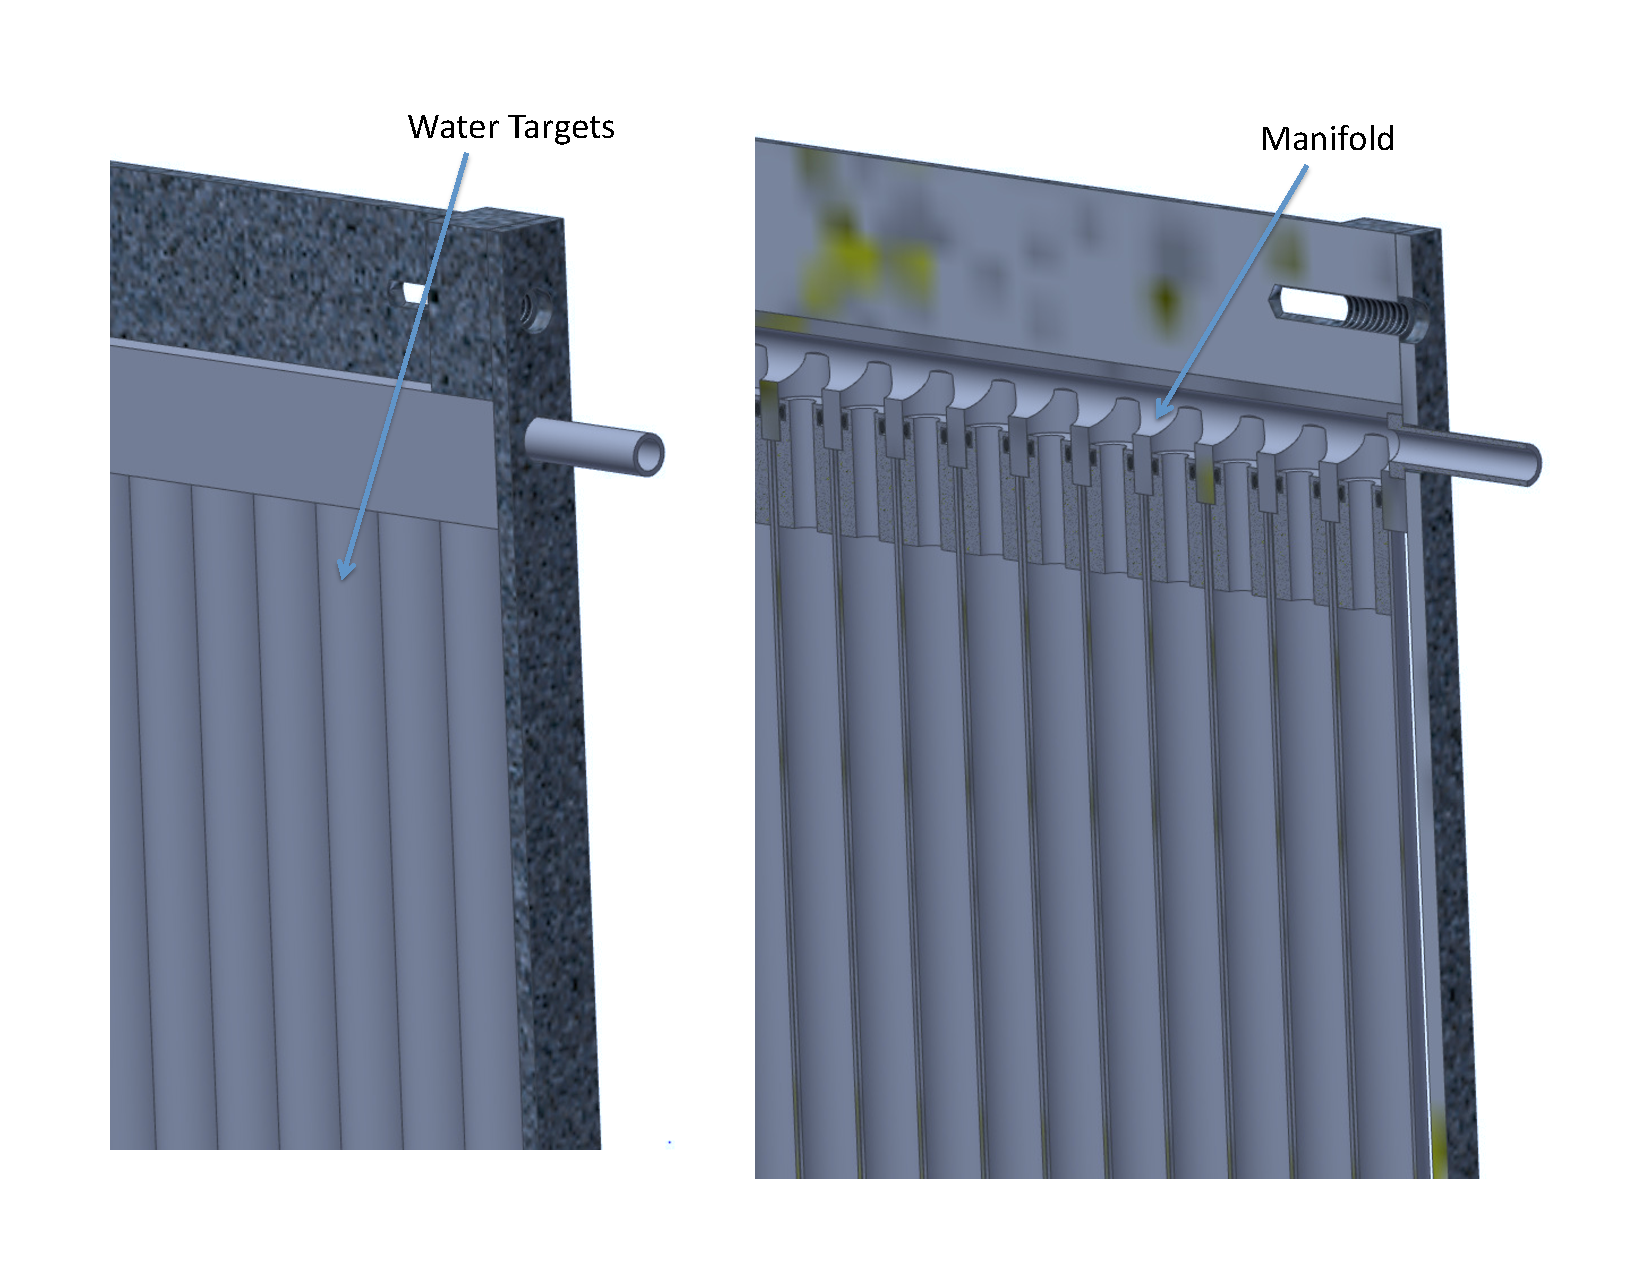
\includegraphics[width=4in,angle=90]{Water_target}
\caption[Schematic drawing of the water or pressurized-argon targets]{\label{STT_targets} Schematic drawing of the water or pressurized-argon targets, 
made from 0.5-in diameter aluminum tubes.}
\end{center}
\end{figure}

\section{Electromagnetic Calorimeter}

An electromagnetic calorimeter 
(ECAL) will surround the tracking volume on all sides and consist of three separate pieces: Forward ECAL, Barrel ECAL, and Backward ECAL. 
The ECAL conceptual design 
%is based on the design of the T2K ECAL and 
consists of 
layers of either 1.75-mm-thick (for the forward ECAL) or 3.5-mm-thick 
(for the barrel and backward ECAL) lead sheets and 2.5-cm-wide by 5-mm-thick 
plastic scintillator bars,
as shown in Figure~\ref{ECAL_detail}. The scintillator layers for the
Forward and Backward ECAL alternate as XYXYXY..., while the scintillator 
layers for the Barrel ECAL are all horizontal along the axis of the magnet.
The Forward ECAL will consist of 58 layers of scintillator bars, where each
bar has dimensions 4~m $\times$ 2.5~cm $\times$ 0.5~cm. The
Backward ECAL will consist of 16 layers of scintillator bars, where each 
bar has the same dimensions, 4~m $\times$ 2.5~cm $\times$ 0.5~cm. The Barrel ECAL will also consist 
of 16 layers of scintillator bars, where each bar has the same dimensions, 
4~m $\times$ 2.5~cm $\times$ 0.5~cm. 

The lead sheets and scintillator bars will be assembled and glued together
into complete modules of dimension 4~m x 4~m x 45~cm for the Forward ECAL and
4~m x 4~m x 15~cm for the Backward ECAL. For the Barrel ECAL the module 
dimensions will be 4~m x 2~m x 15~cm. Two Barrel modules are placed end to
end along the sides of the inner surface of the magnet (16 Barrel modules
total) to provide full coverage of the barrel region.
The total numbers of scintillator bars in the
Forward, Backward, and Barrel ECAL are 9280, 2560, and 20,480, respectively, 
for a total of 32,320 bars. 

The scintillator bars will be extruded with 
holes in the middle of each bar. The
holes will then be fitted with 0.7-mm-diameter Kuraray wavelength-shifting (WLS) fibers.
The fibers will be read out by SiPM photosensors at each end, making the number of 
readout channels twice the number of scintillator bars 
for a total of 64,640. The total mass of scintillator is 16.16 tons, the total mass of Pb is 110 tons, and
the total length of fiber is 129.3 km.
Specifications for the ECAL are shown in Table \ref{ECAL_specs}.

\begin{figure}
\begin{center}
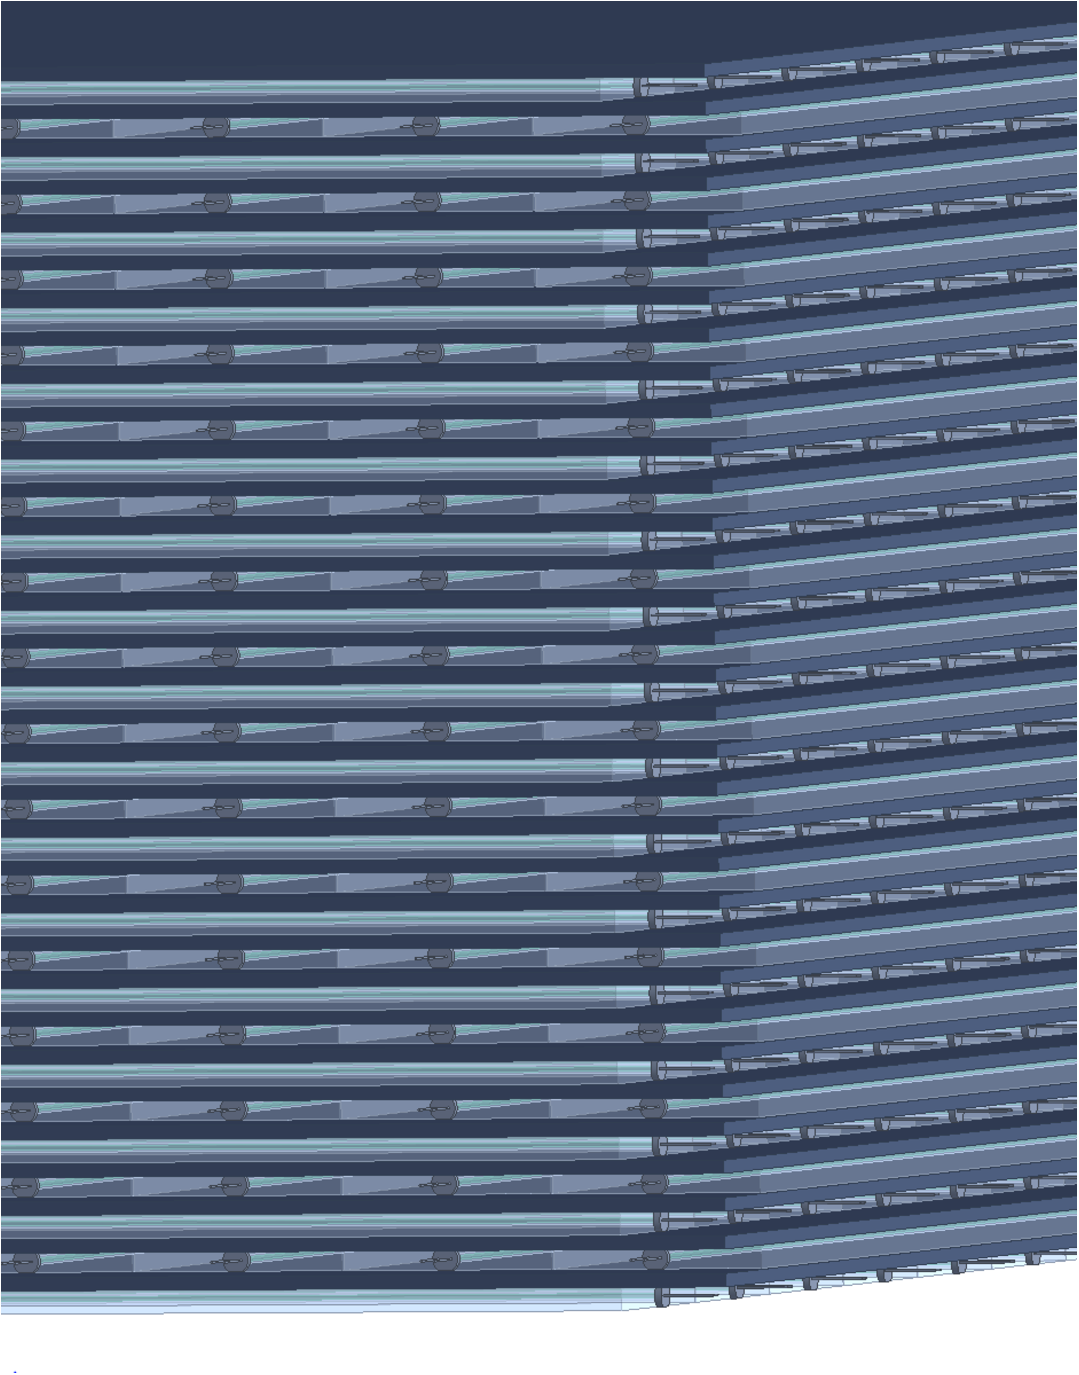
\includegraphics[width=3.0in,angle=90]{ECAL_detail}
\caption[Schematic drawing of the ECAL]{\label{ECAL_detail} Schematic drawing of the ECAL, which is made up of alternating planes
of plastic scintillator and Pb sheets.}
\end{center}
\end{figure}

\begin{table}
\centering
  \caption{\label{ECAL_specs} ECAL specifications.}
  \begin{tabular}{| l | l |}
    \hline
Item&Specification \\
    \hline
Scintillator Bar Geometry & 4m x 2.5cm x 0.5cm \\
Number of Forward ECAL Scintillator Bars & 9280 \\
Forward ECAL Pb thickness & 1.75mm \\
Number of Forward ECAL Layers & 58 \\
Number of Forward ECAL Radiation Lengths & 18 \\
Dimensions of Forward ECAL Module & 4m x 4m x 45cm \\
Number of Barrel ECAL Scintillator Bars & 20,480 \\
Barrel ECAL Pb thickness & 3.5mm \\
Number of Barrel ECAL Layers & 16 \\
Number of Barrel ECAL Radiation Lengths & 10 \\
Number of Barrel ECAL Modules & 16 \\
Dimensions of Barrel ECAL Modules & 4m x 2m x 15cm \\
Number of Backward ECAL Scintillator Bars & 2560 \\
Backward ECAL Pb thickness & 3.5mm \\
Number of Backward ECAL Layers & 16 \\
Number of Backward ECAL Radiation Lengths & 10 \\
Dimensions of Backward ECAL Module & 4m x 4m x 15cm \\
Total Length of 0.7mm Diameter WLS Fiber & 129.3km \\
Total Number of Scintillator Bars & 32,320 \\
Total Number of Electronics Channels & 64,640 \\
Total Mass of Scintillator & 16,160 kg \\
Total Mass of Pb & 110,000kg \\
     \hline
  \end{tabular}
\end{table}

\section{Dipole Magnet} 

The STT and ECAL modules will reside inside a 0.4-T dipole 
magnet for the measurement of particle momentum and charge. 
The magnet will have inner dimensions (inside the coils) 
4.5-m wide $\times$ 4.5-m high $\times$ 8.0-m long. The 
magnet 
%is modeled after the CERN 
%UA1 magnet with 
has four vertical Al coils, stacked horizontally, producing a horizontal magnetic 
field. The return yoke will be divided into two halves along the 
longitudinal center line to allow the magnet to be opened to service the
detector inside, as shown in Figure~\ref{STT_schematic}. 
Each half yoke will be built
from eight ``C'' sections, and the thickness of the 
magnet steel will be 60~cm, consisting of 6
$\times$ 10-cm-thick plates. The magnet power requirement with Al coils is $\sim 2.4$~MW,
corresponding to 6~kA at 400~V. The water flow required for cooling is 20~l/s.
The Dipole Magnet specifications are shown in Table \ref{Magnet_specs}.

The momentum resolution is dominated by multiple scattering in the STT. The momentum resolution is, therefore, given by 
$\delta p/p = 0.053/\sqrt(LX_0)B$. For B = 0.4T, L = 3m, and $X_0 = 4$m, the
expected momentum resolution is $\sim 3.8\%$. 

\begin{table}
\centering
  \caption{\label{Magnet_specs} Dipole Magnet specifications.}
  \begin{tabular}{| l | l |}
    \hline
Item&Specification \\
    \hline
Inner Dimensions & 4.5m x 4.5m x 8.0m \\
Magnetic Field & 0.4 T \\
Number of ``C'' Sections & 16 \\
Thickness of Steel in the ``C'' Sections & 60cm \\
Number of Coils & 4 \\
Magnet Current & 6 kA \\
Magnet Voltage & 400 V \\
Magnet Power Requirements & 2.4 MW \\
Water Flow for Cooling & 20 l/s \\
     \hline
  \end{tabular}
\end{table}

\section{Muon Identifier}
\label{sec:muid}

%\fixme{Lots of repetition here; can we just say 'like the LArTPCT MuID except for these differences...?}
%I would rather have the repetition so that it is a stand-alone section. BL}
The sides and ends of the dipole magnet will be instrumented
with a muon identifier
detector (MuID) that will distinguish muons from hadrons by their ability 
to penetrate the iron without showering or interacting.
The MuID will consist of 32 RPC planes
interspersed between 2 $\times$ 10-cm-thick steel plates of the 
dipole magnet and between 20-cm-thick steel plates at the upstream and
downstream ends of the magnet. 
The MuID is only meant to provide %the 
identification of the 
muon; the muon momentum %itself 
will be measured by the STT inside the 
magnetic field. A schematic drawing of the MuID 
interspersed in the magnet steel is shown in Figure~\ref{FGT_MuID}.

The dimensions of the barrel- and end-RPC planes will be $\sim$ 2.5~m $\times$ 8~m and
6~m $\times$ 6~m, respectively. The end-RPC planes are divided into 
sub-planes of dimensions 1~m $\times$ 2~m. The barrel-RPC planes are divided into
sub-planes A, B, C, D, and E, as shown in Figure \ref{MuID_detail}. 
The downstream MuID will contain 5 steel planes of 
overall dimension
6 x 6 x 0.2 m$^3$ (283.5 tons)
and 5 RPC planes, while the upstream MuID will contain 3 steel
planes (170.1 tons) of dimension 6 x 6 x 0.2 m$^3$ and 3 RPC planes. The barrel MuID will contain
24 planes (3 layers x 8 sides) of RPCs. The RPCs will have a total thickness 
of 15 mm and a gap width of 2 mm. One possible gas mixture would be composed, for example,
of Ar (75\%), tetraflouroethane (20\%), isobutane (4\%),
and sulphurhexaflouride (1\%). Each side of the RPC will have 7 mm pitch strips, which will
allow both an X and a Y measurement. The total number of strips and electronic channels will
be 86,402. A schematic drawing of an RPC is shown in Figure~\ref{FGT_RPC}.
MuID specifications are shown in Table \ref{MID_specs}.

\begin{figure}[htp]
\begin{center}
\includegraphics[width=5in,angle=90]{MuID_schematic}
\caption{\label{FGT_MuID} Schematic drawing of the MuID (blue modules) interspersed in the magnet steel.}
\end{center}
\end{figure}

\begin{figure}[htp]
\begin{center}
\includegraphics[width=5in,angle=90]{MuID_detail}
\caption{\label{MuID_detail} Schematic drawing of the barrel MuID (with dimensions) 
interspersed in the magnet steel.}
\end{center}
\end{figure}

\begin{figure}[htp]
\begin{center}
\includegraphics[width=3in,angle=90]{RPC_schematic.eps}
\caption{\label{FGT_RPC} Schematic drawing of an RPC.} 
%from Jiawen Zhang, 9th ACFA ILC Physics
%and Detector Workshop \& ILC GDE Meeting, Feb. 4-7, 2007, IHEP, Beijing.}
\end{center}
\end{figure}

\begin{table}
\centering
  \caption{\label{MID_specs} MuID specifications.}
  \begin{tabular}{| l | l |}
    \hline
Item&Specification \\
    \hline
Number of Barrel RPC Sub-Planes A & 56 \\
Dimensions of Barrel RPC Sub-Planes A &  1.44m x 2m \\
Number of Barrel RPC Sub-Planes B & 16 \\
Dimensions of Barrel RPC Sub-Planes B &  1.18m x 2m \\
Number of Barrel RPC Sub-Planes C & 32 \\
Dimensions of Barrel RPC Sub-Planes C &  1.12m x 2m \\
Number of Barrel RPC Sub-Planes D & 16 \\
Dimensions of Barrel RPC Sub-Planes D &  0.895m x 2m \\
Number of Barrel RPC Sub-Planes E & 16 \\
Dimensions of Barrel RPC Sub-Planes E &  0.546m x 2m \\
Number of Barrel RPC Planes & 24 \\
Dimensions of Barrel RPC Planes & 2.5m x 8m \\
Number of End RPC Sub-Planes & 144 \\
Dimensions of End RPC Sub-Planes & 1m x 2m \\
Number of Downstream End RPC Planes & 5 \\
Number of Upstream End RPC Planes & 3 \\
Dimensions of End RPC Planes & 6m x 6m \\
Mass of Downstream Steel Planes & 283,500 kg \\
Mass of Upstream Steel Planes & 170,100 kg \\
RPC Thickness & 1.5cm \\
Distance Between RPC Strips & 7mm \\
Total Number of RPC Strips and Electronics & 86,402 \\
     \hline
  \end{tabular}
\end{table}

\section{Instrumentation}

The instrumentation includes readout-electronics for the sub-detectors
and the slow-control of the sub-detector, involving monitoring the humidity, 
temperature, gas pressure, etc.
There is considerable synergy in the information gathered in the STT, ECAL and MuID.
Both STT and ECAL are required to measure the total charge and time associated with a 
given hit. The MuID RPCs are required to provide the position and time associated with 
a traversing-track. Similarly, the slow control of the sub-detectors
share many features. 
A brief description of the sub-detector instrumentation is presented below, while
Table \ref{elect_ch} summarizes the number of electronics channels for each of the
three detector systems. 

\begin{table}
\centering
  \caption{\label{elect_ch} The number of electronics channels for each of the
three detector systems.}
  \begin{tabular}{| c | c |}
    \hline
Detector&Number of Electronics Channels \\
    \hline
STT & 247,808 \\
ECAL & 64,640 \\
MuID & 86,402 \\
     \hline
  \end{tabular}
\end{table}

\subsection{Readout Electronics for the STT}

To minimize ambiguity in assigning hits to a track, the straw tubes will be readout 
at both ends. The readout electronics will be similar to the ATLAS TRT electronics. 
Front-end (FE) boards, mounted on the STT frame, will provide amplification, shaping, 
and baseline restoration. The FE will be an 8-channel analogue ASIC. A 
subsequent 16-channel ASIC will perform the drift-time measurement ($\sim 3$ ns binning). 
The TR and dE/dx measurements will be performed with an ADC connected to the FE-ASIC.
In summary, the STT readout will digitize the time, total charge, and 
transition-radiation associated with a hit.

\subsection{Readout Electronics for the ECAL}

The silicon photomultipliers (SiPMs) receive light on either end of
the WLS fiber 
instrumenting the scintillation bars. The readout of the SiPMs will provide the total 
pulse-height and time associated with energy (light) deposited in the scintillator bars. 
For a given particle traversing the ECAL, e.g. a photon, the energy (dynamic) range 
should cover from about 50 MeV to 10 GeV. What this means in terms of
the readout of a single SiPM will be determined from a detailed Monte Carlo study 
and confirmed by test-beam measurements.
The time resolution for a particle traversing the ECAL should be $\sim 1$ ns.

\subsection{Readout Electronics for the MuID}

The MuID RPCs will provide the position and time information. The required position 
resolution is about 0.6 mm, and the time-resolution is about 2 ns.

\subsection{Monitoring Humidity \& Temperature in the STT, ECAL, MuID, and Magnet}

Humidity is inimical to all sub-detectors in the FGT. To maintain a low-level of 
humidity and to maintain a desired temperature, both STT and ECAL sub-detectors
will have dry nitrogen circulating within their outer layers. A similar arrangement 
might be made for the RPCs as well. Furthermore, magnet coils are cooled by water, 
while the magnet yokes are instrumented with RPCs. Thus, a continuous control of 
humidity in all these detectors is needed.
Just as humidity, temperature must be continuously monitored in all of the sub-detectors.

\subsection{Monitoring Gas Leaks in the STT and MuID}

Gas-leaks need to be monitored in the STT and MuID.
The STT will employ Xe gas, which is expensive and, hence, will be recirculated. It is 
most essential to ensure that Xe is not leaking. The requirement for leaks is less 
stringent for the RPC. 

\subsection{Monitoring Cooling-Water Flow in the Magnet}

The water flow (pressure gradient) must be continuously monitored.

\subsection{Monitoring Voltage and Current}

All power sources instrumenting the FGT and its readout need to be monitored for 
appropriate voltage and current.

\vfill\eject

\end{document}

